\documentclass[12pt]{article}
\usepackage[scale=0.75]{geometry}
\usepackage{graphicx}
\usepackage{listings}
\lstset{language=Matlab, breaklines=true}
\renewcommand*{\familydefault}{\sfdefault}

\begin{document}

\title{Financial Engineering II\\Lab Assignment 8}
\author{Gajula Jyothendranadh Sai, 11012311}
\date{\today}
\maketitle
\tableofcontents
\newpage

\section{Plot of volatility against period length}
  \begin{center}
    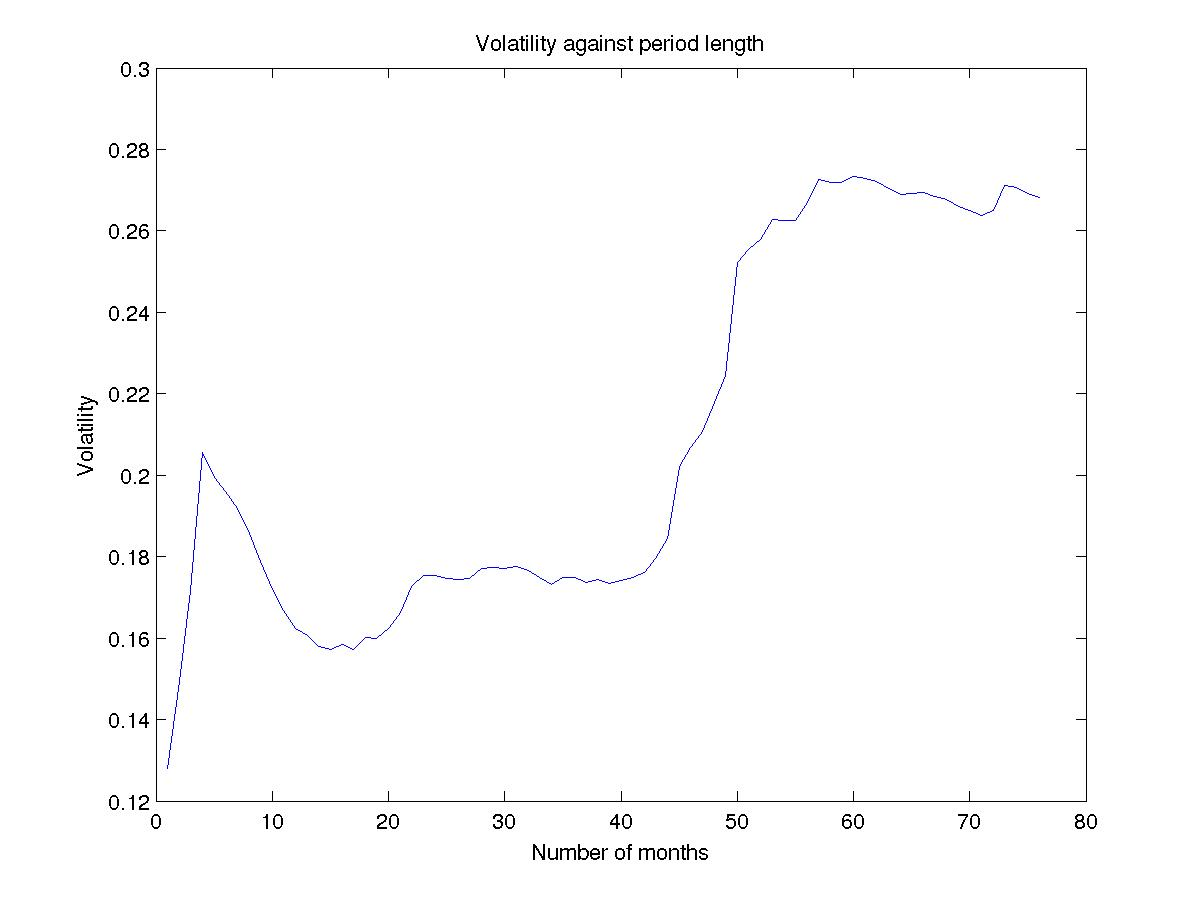
\includegraphics[width=4in]{volatility.jpg}
  \end{center}

\section{Option prices against period length}
  \subsection{Call option prices}
    \begin{center}
      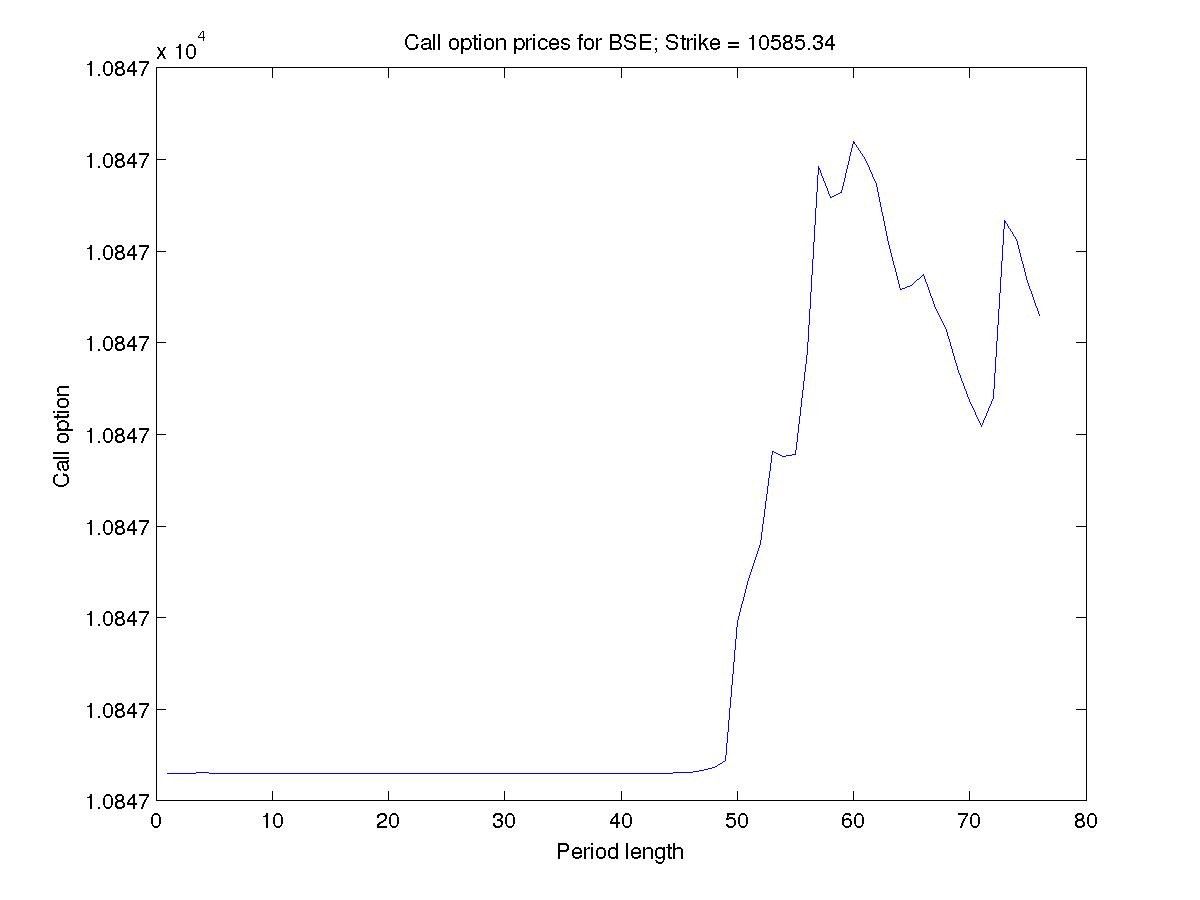
\includegraphics[width=5in]{call_strike1.jpg}
      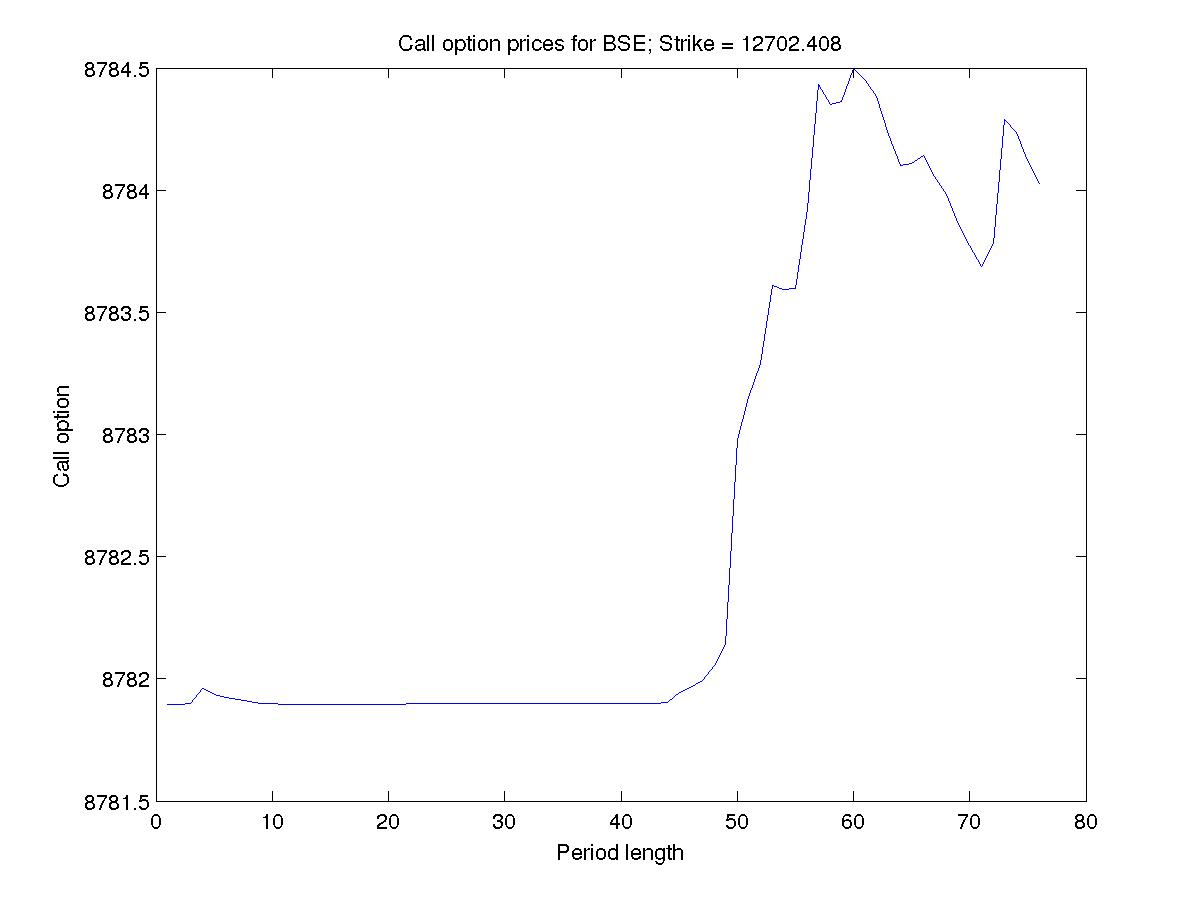
\includegraphics[width=5in]{call_strike2.jpg}
      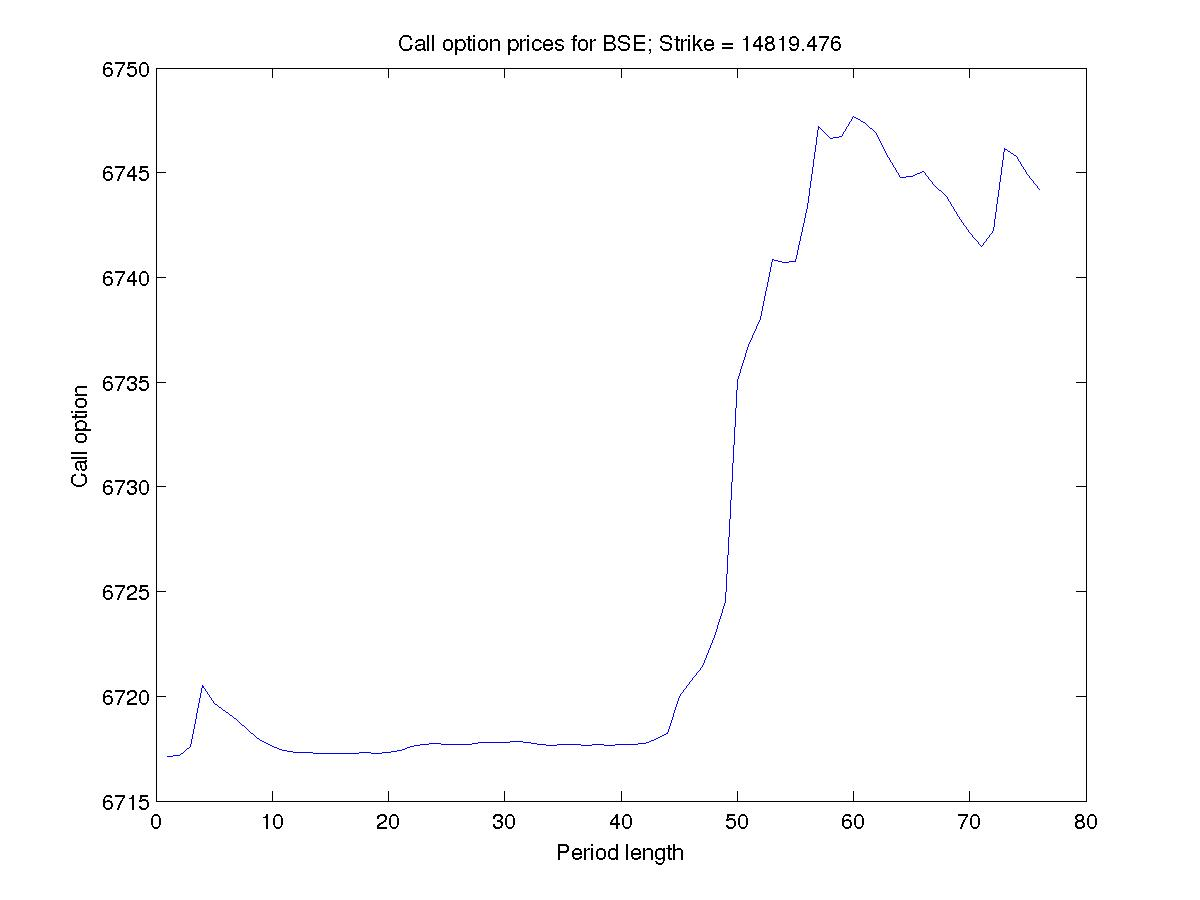
\includegraphics[width=5in]{call_strike3.jpg}
      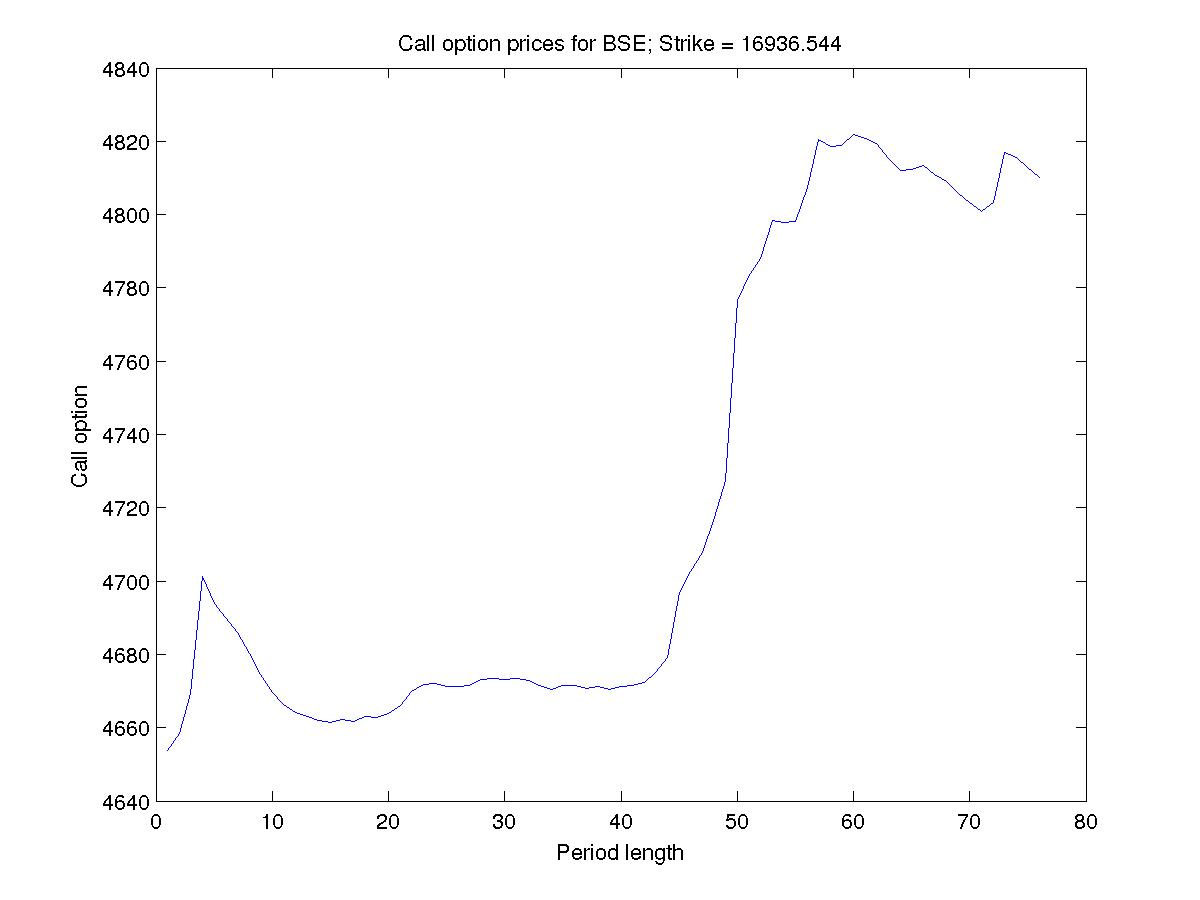
\includegraphics[width=5in]{call_strike4.jpg}
      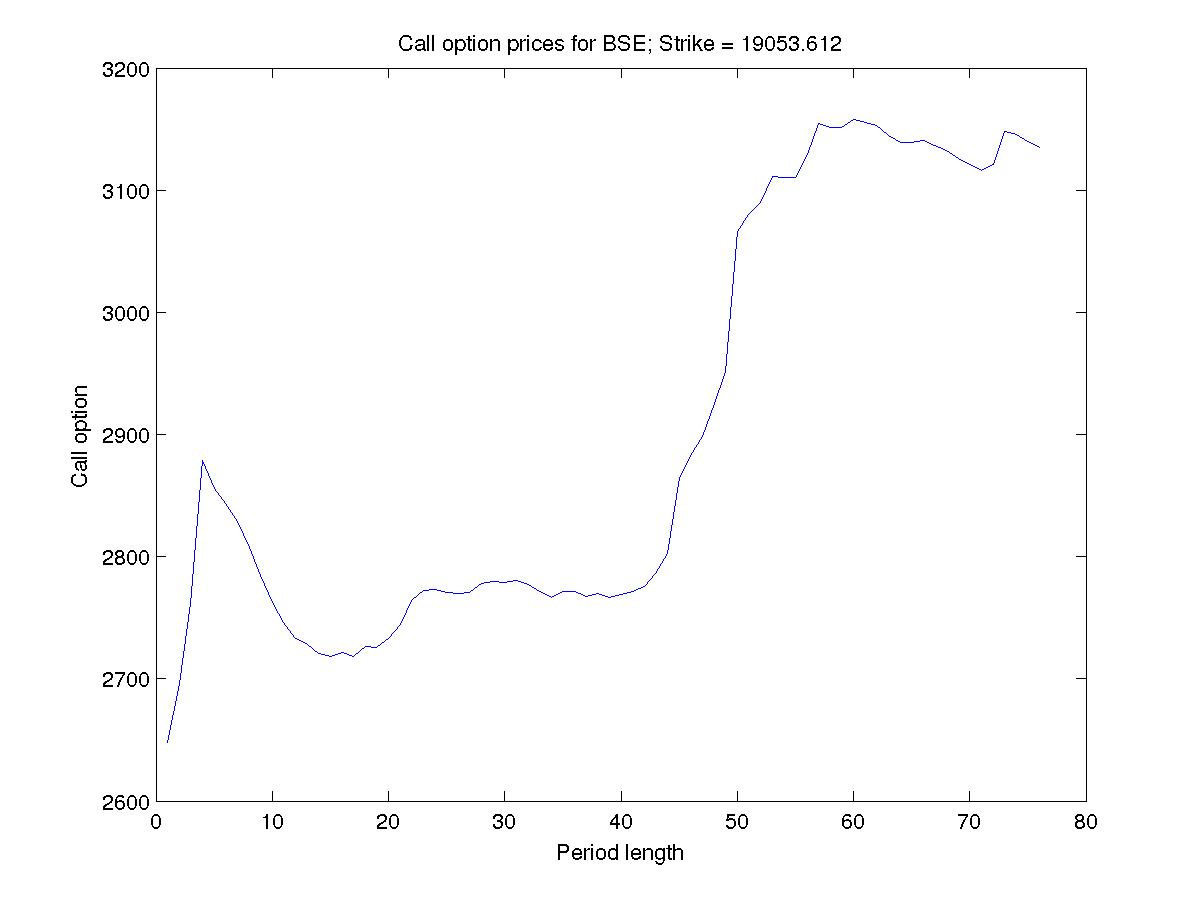
\includegraphics[width=5in]{call_strike5.jpg}
      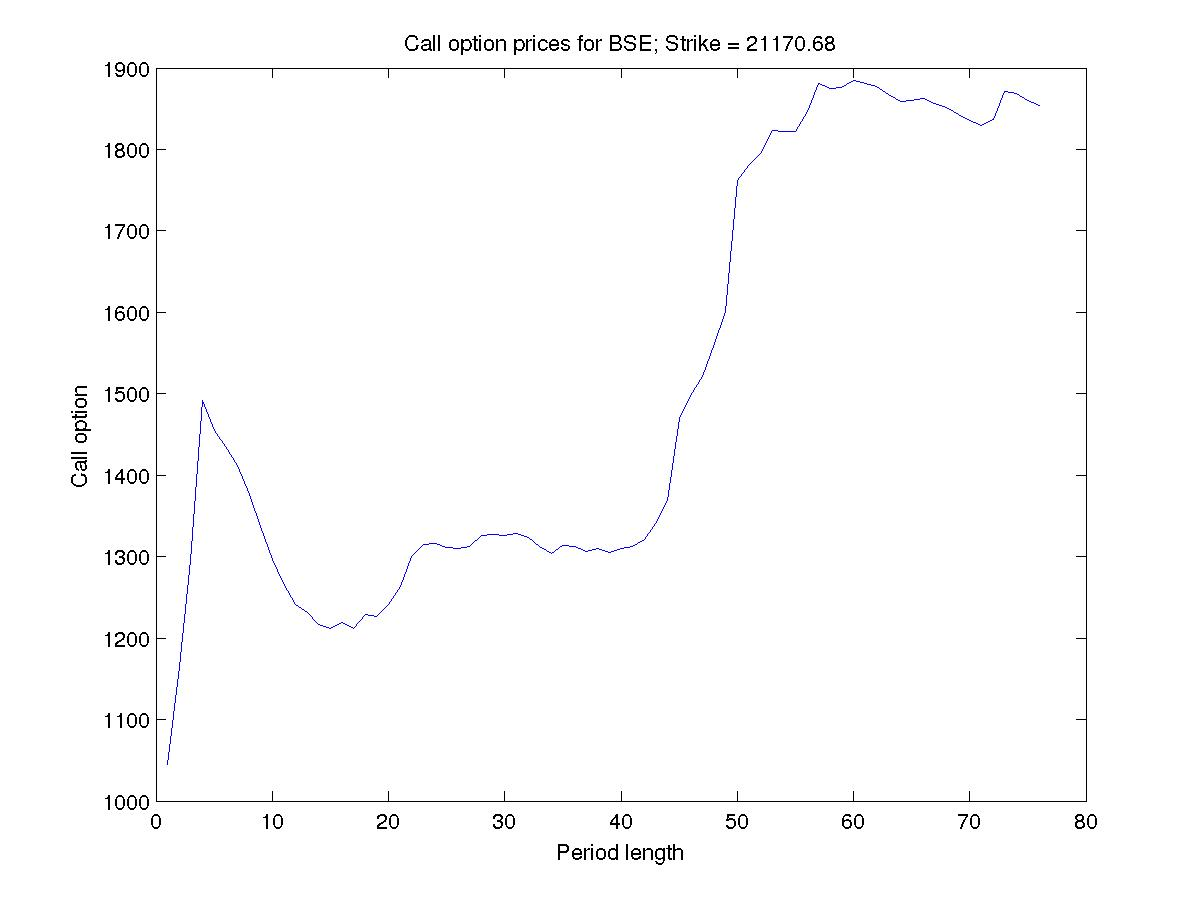
\includegraphics[width=5in]{call_strike6.jpg}
      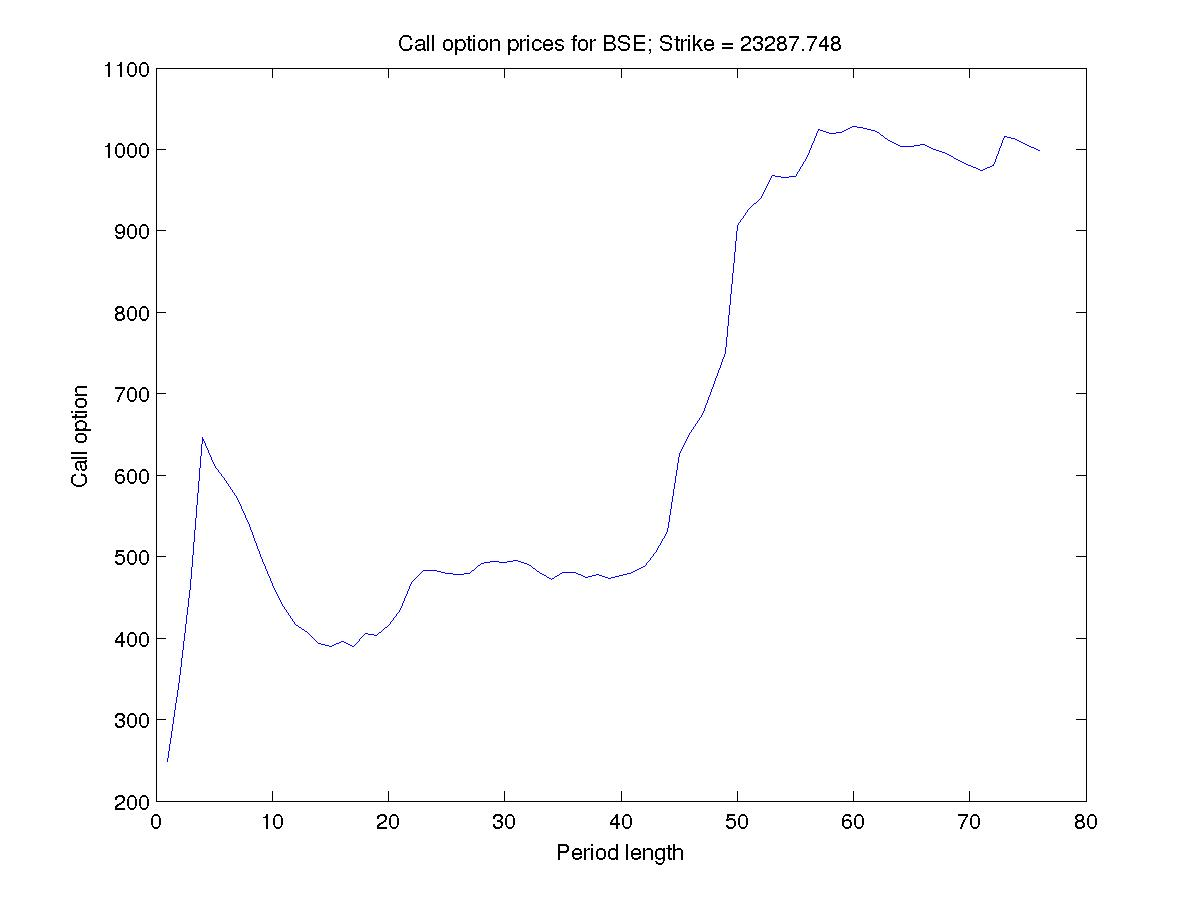
\includegraphics[width=5in]{call_strike7.jpg}
      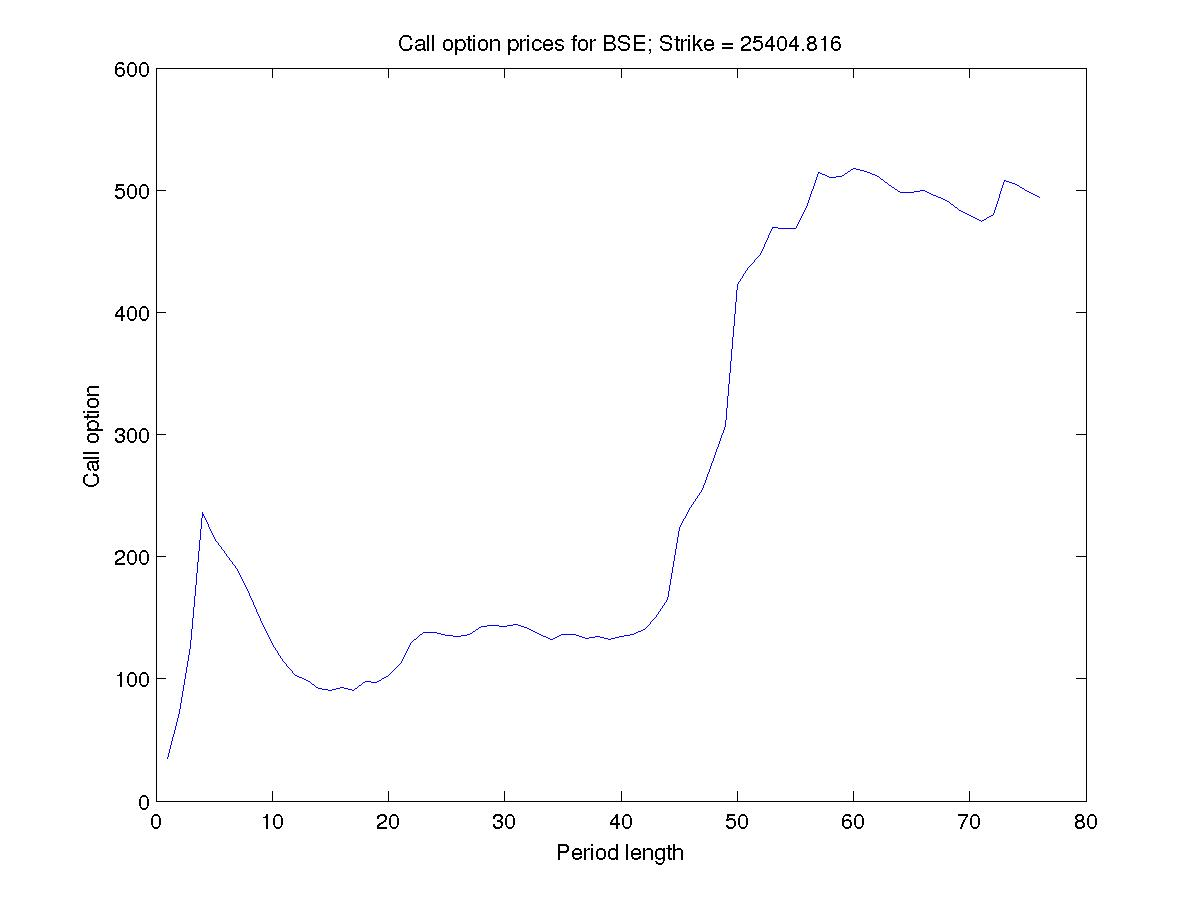
\includegraphics[width=5in]{call_strike8.jpg}
      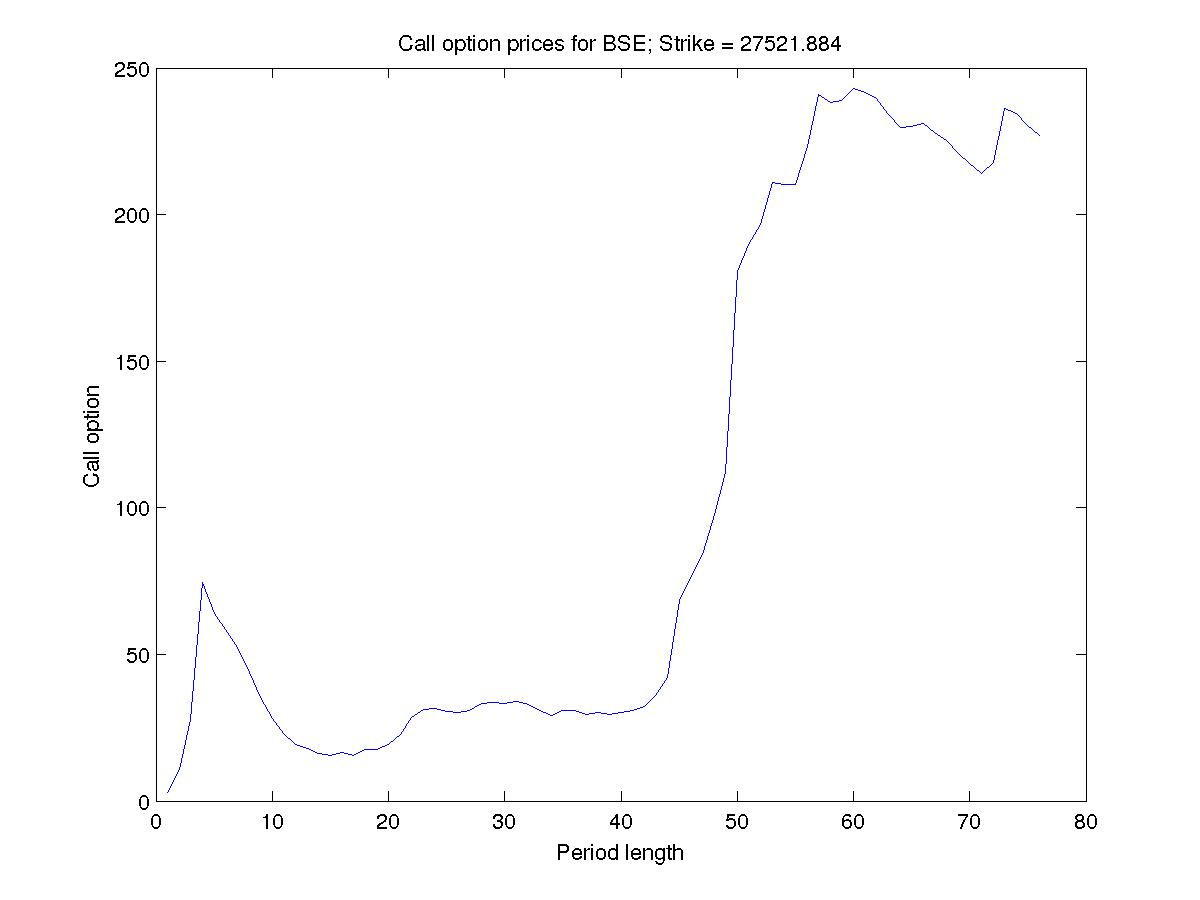
\includegraphics[width=5in]{call_strike9.jpg}
      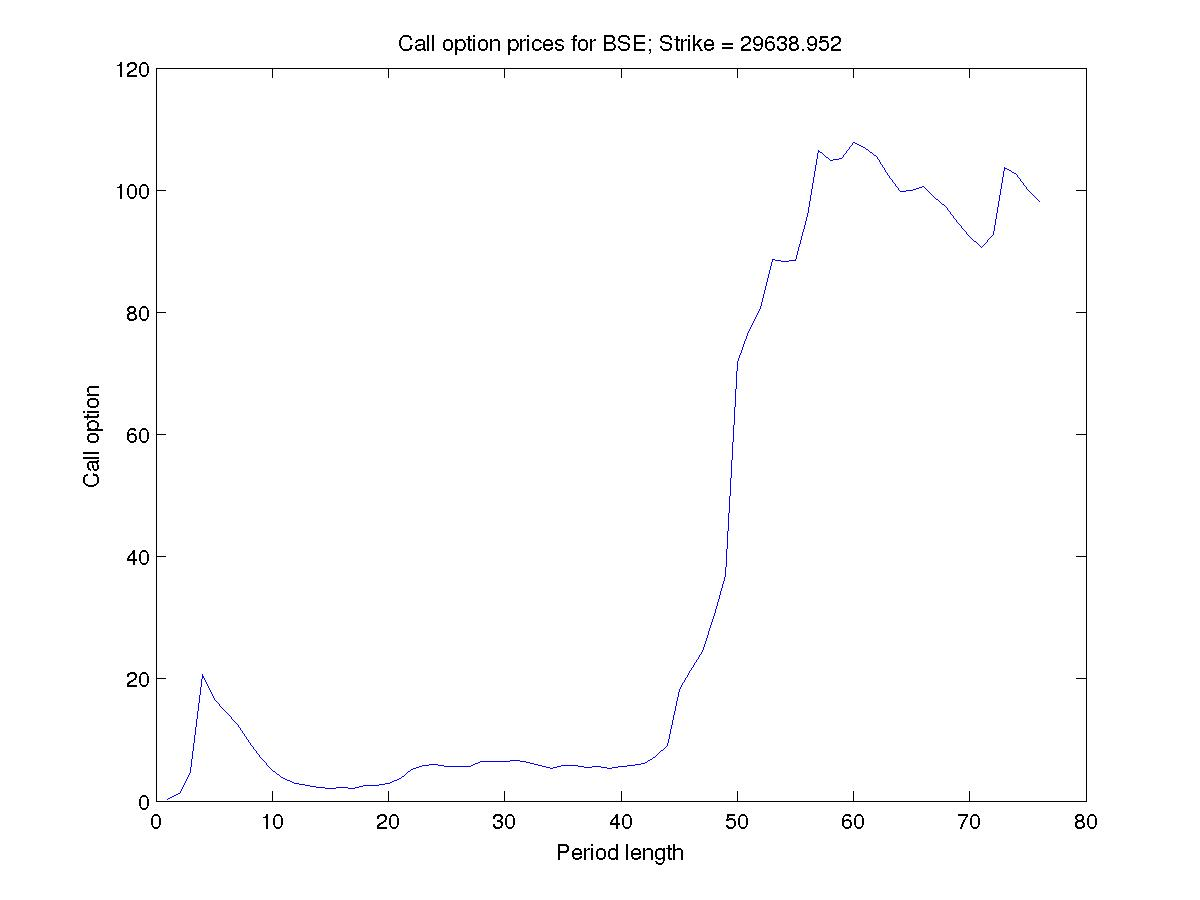
\includegraphics[width=5in]{call_strike10.jpg}
    \end{center}
  \subsection{Put option prices}
    \begin{center}
      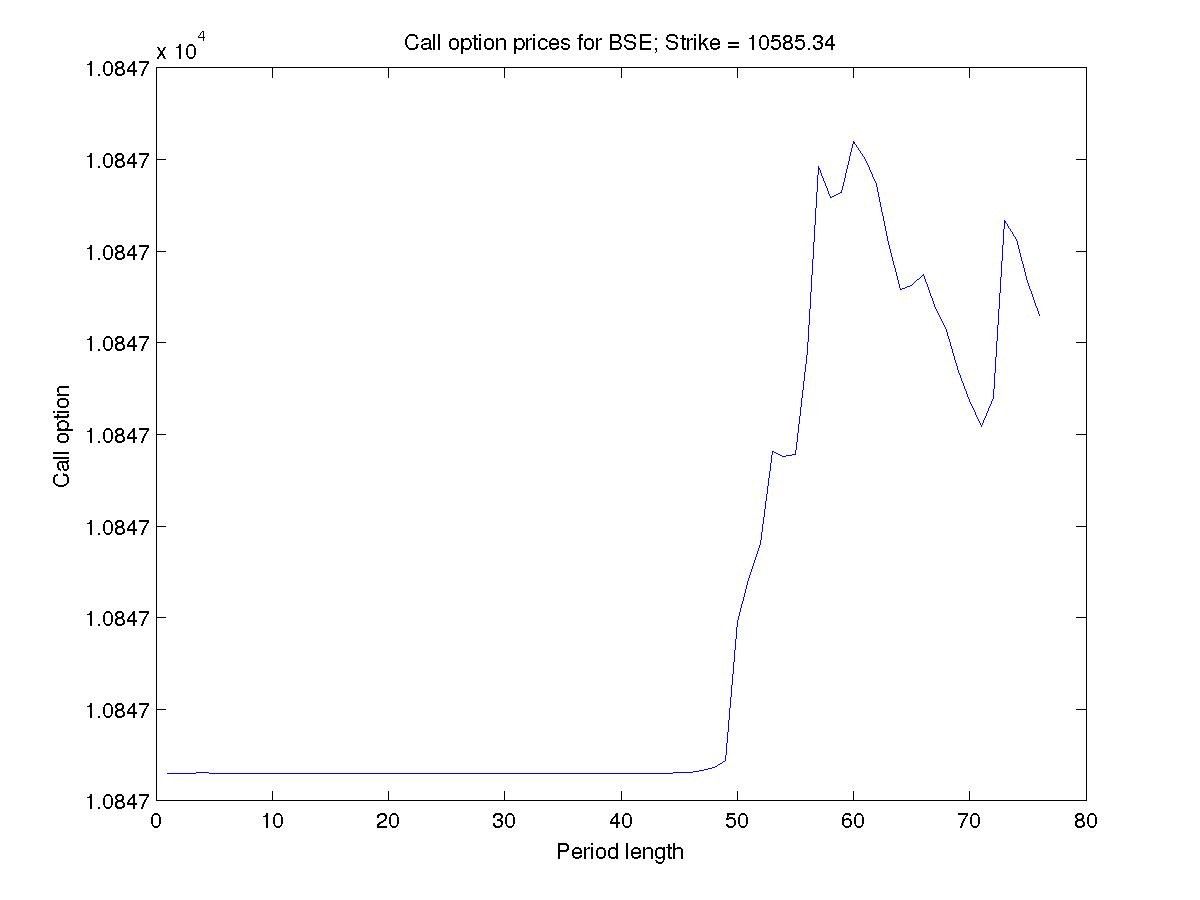
\includegraphics[width=5in]{put_strike1.jpg}
      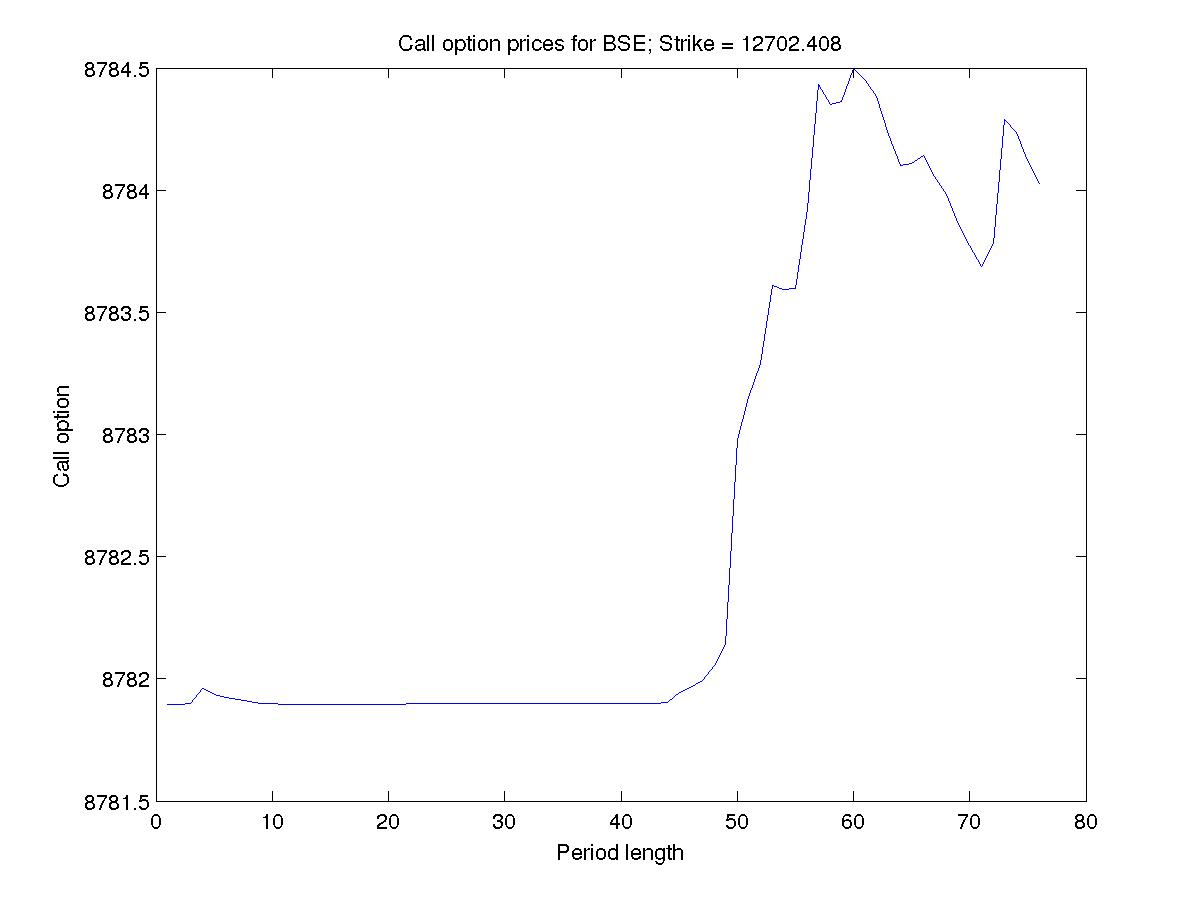
\includegraphics[width=5in]{put_strike2.jpg}
      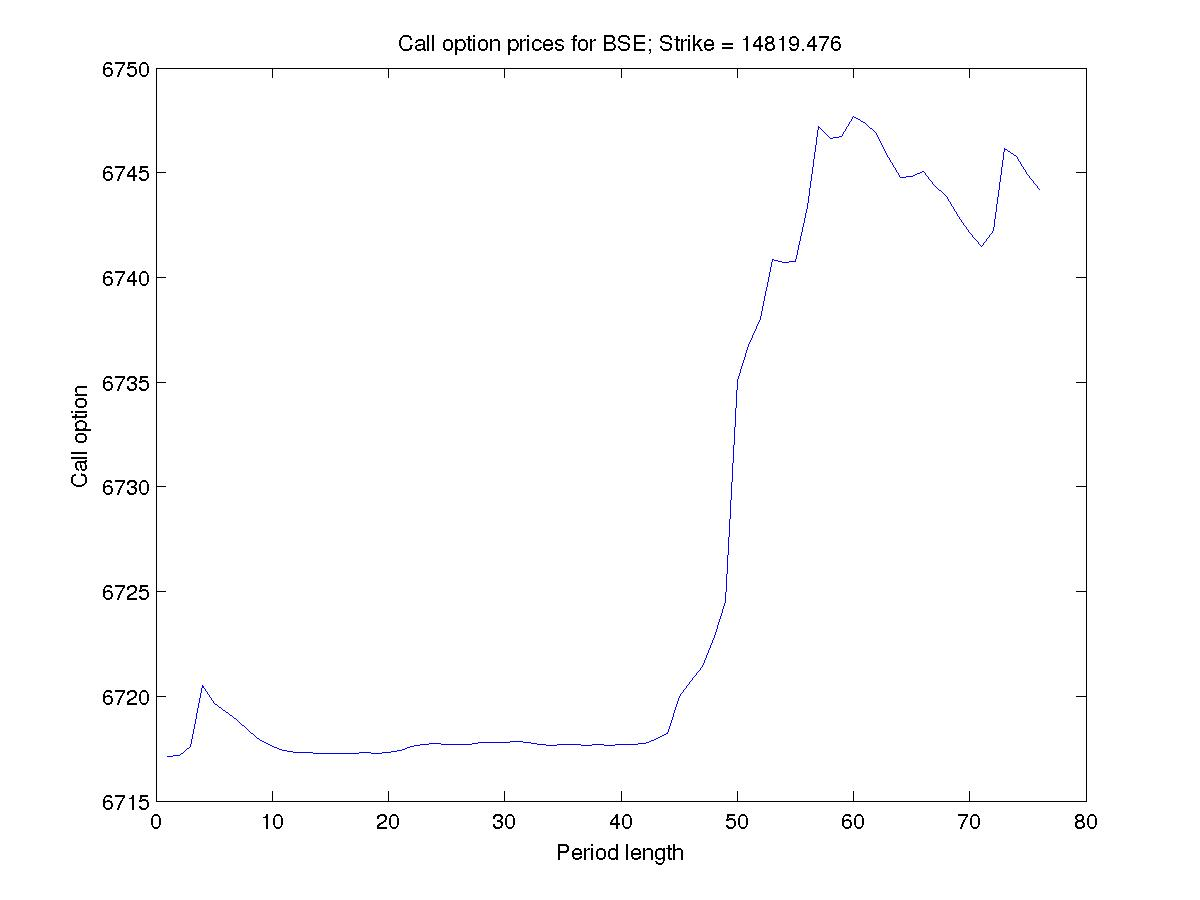
\includegraphics[width=5in]{put_strike3.jpg}
      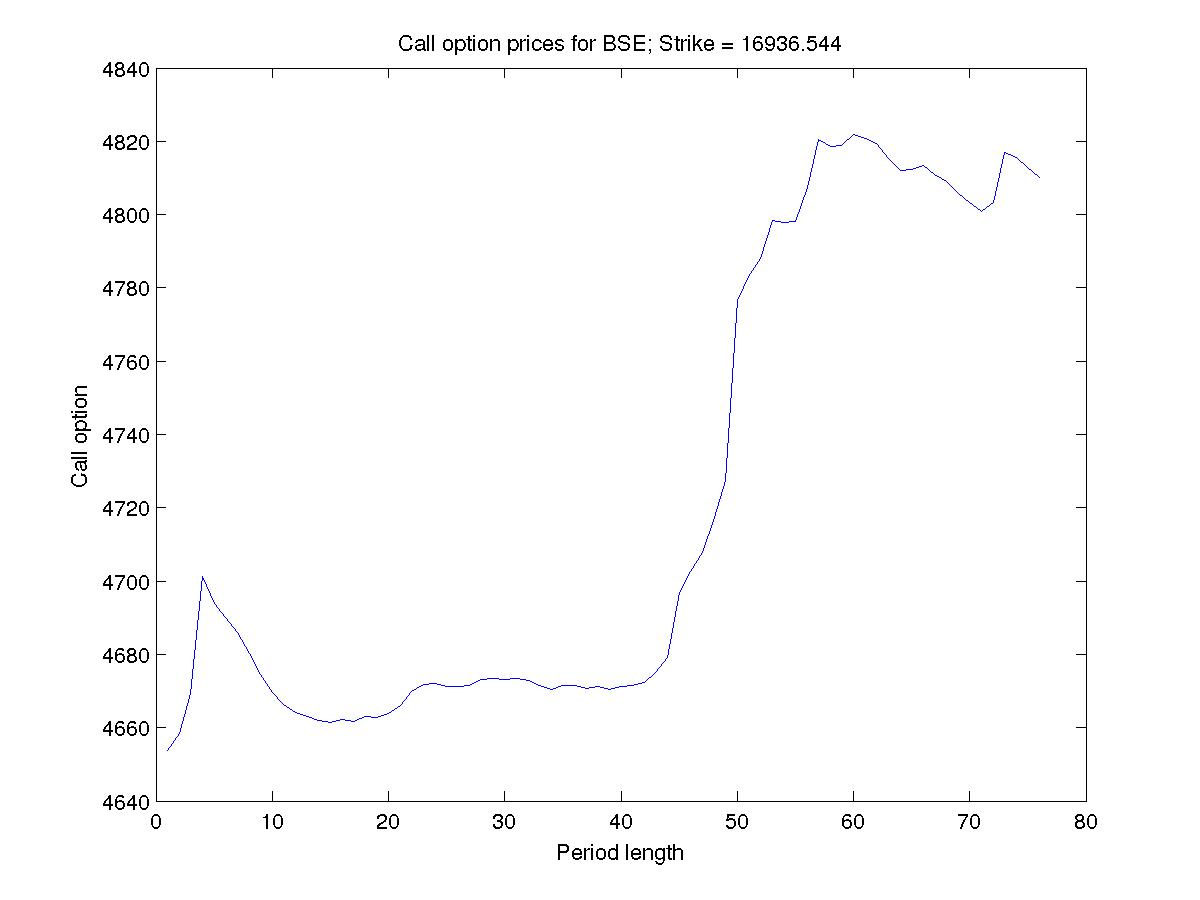
\includegraphics[width=5in]{put_strike4.jpg}
      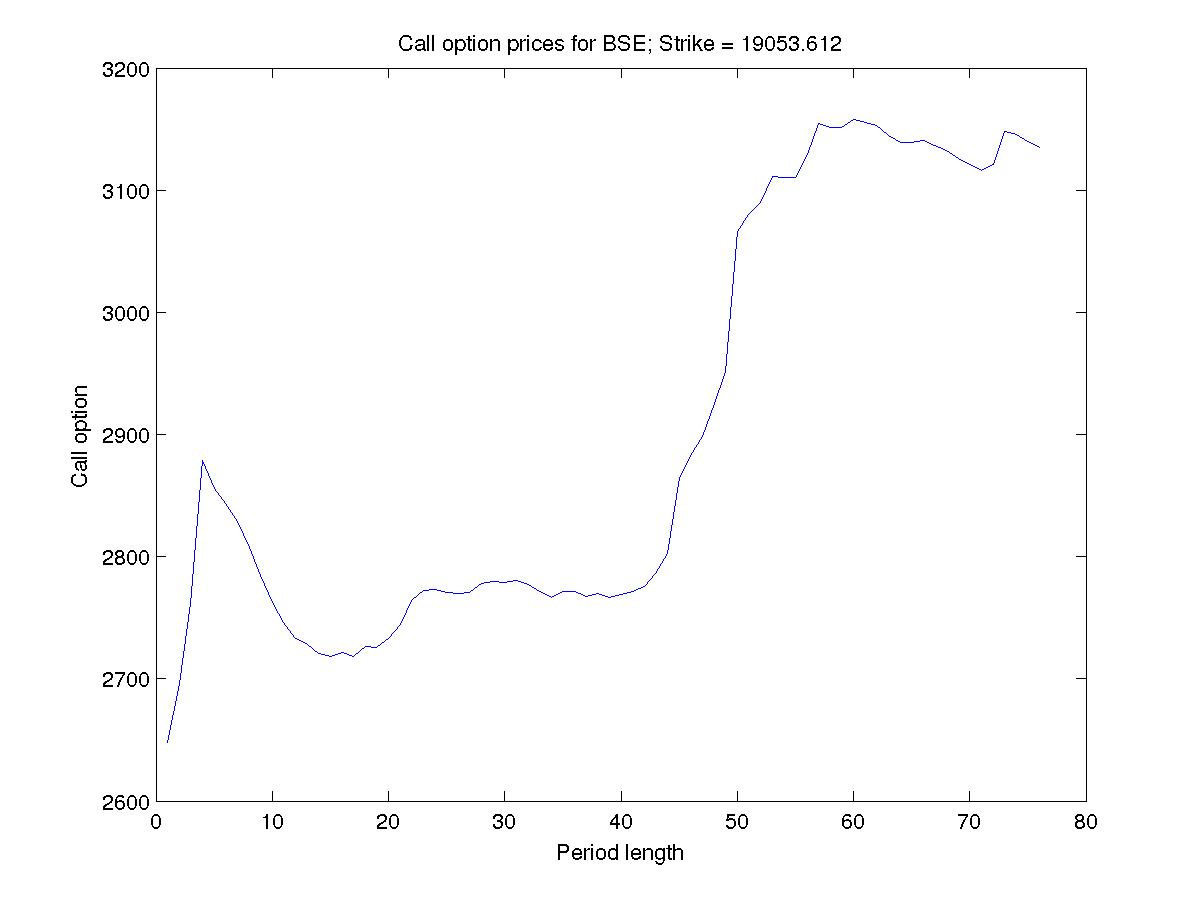
\includegraphics[width=5in]{put_strike5.jpg}
      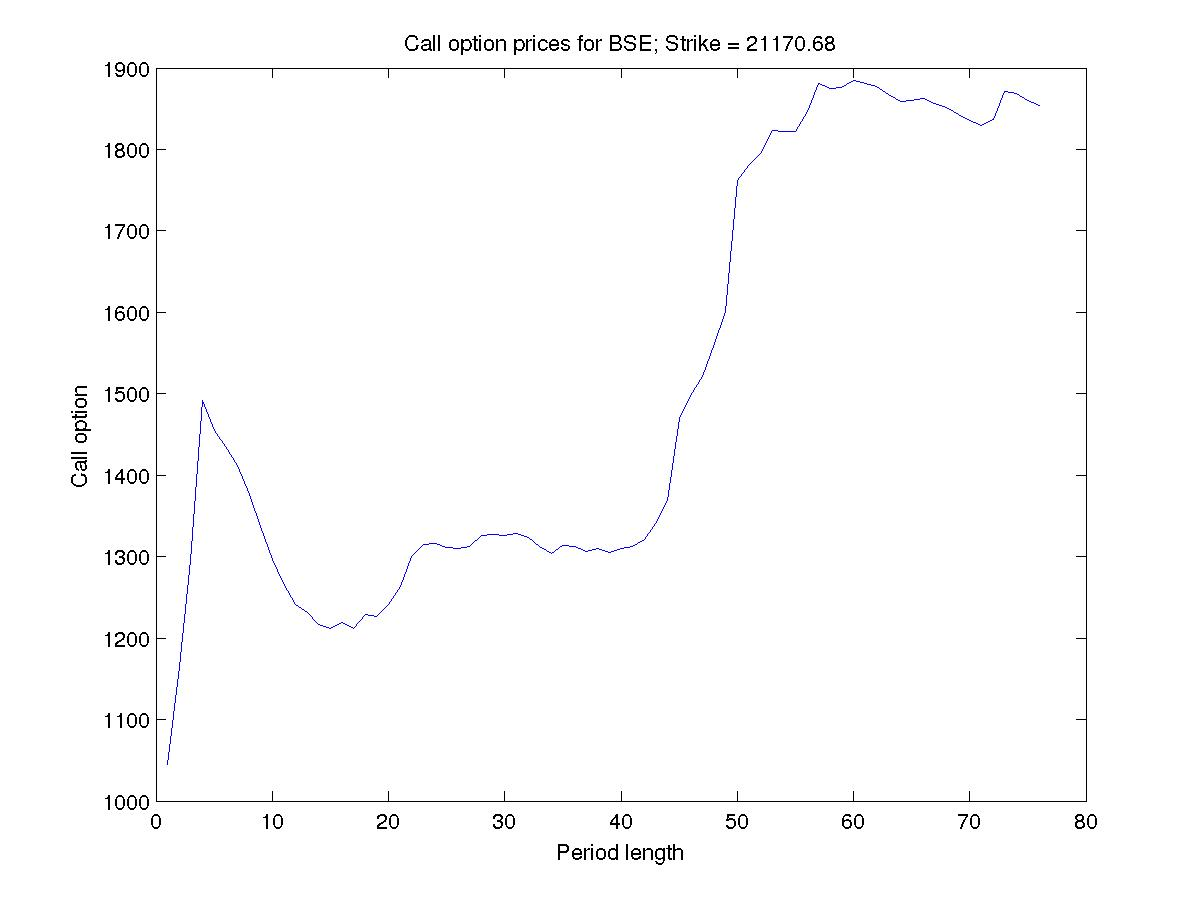
\includegraphics[width=5in]{put_strike6.jpg}
      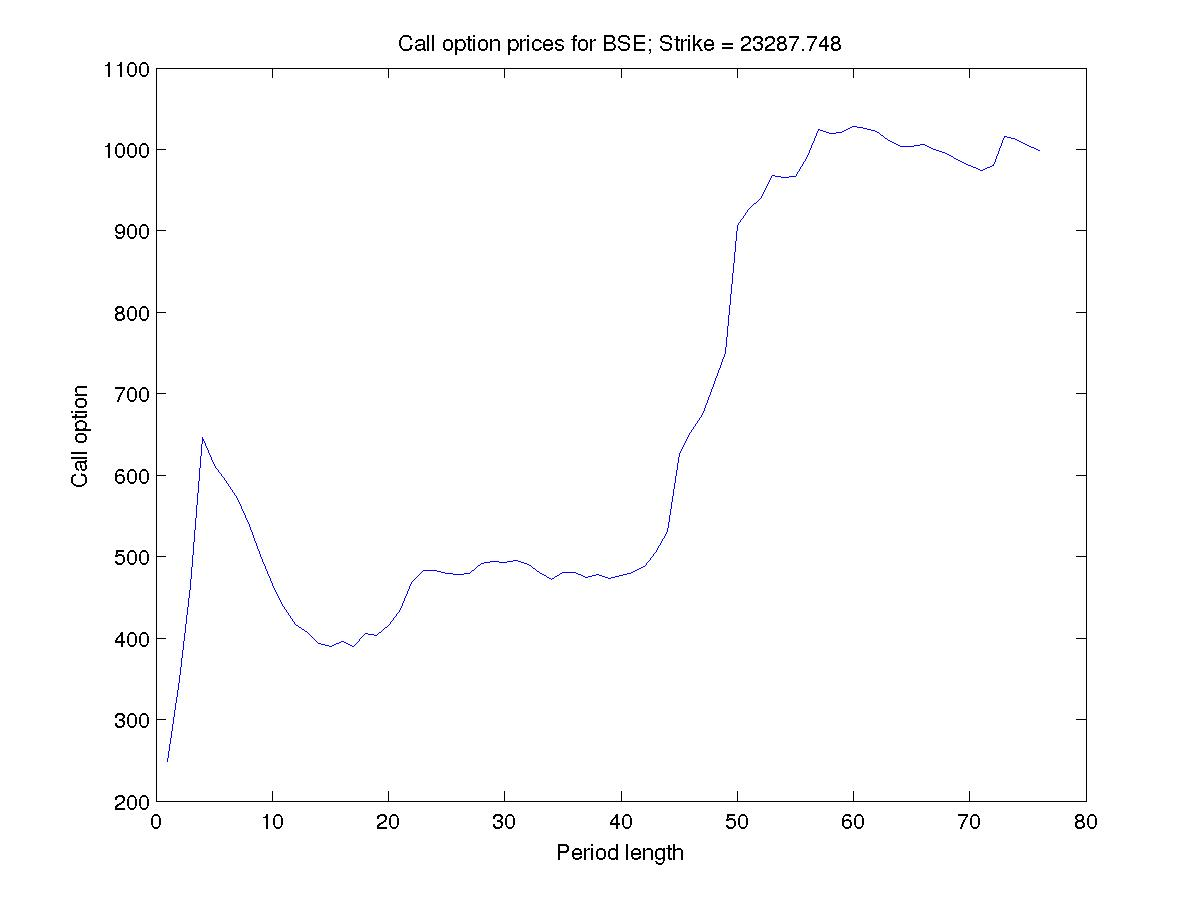
\includegraphics[width=5in]{put_strike7.jpg}
      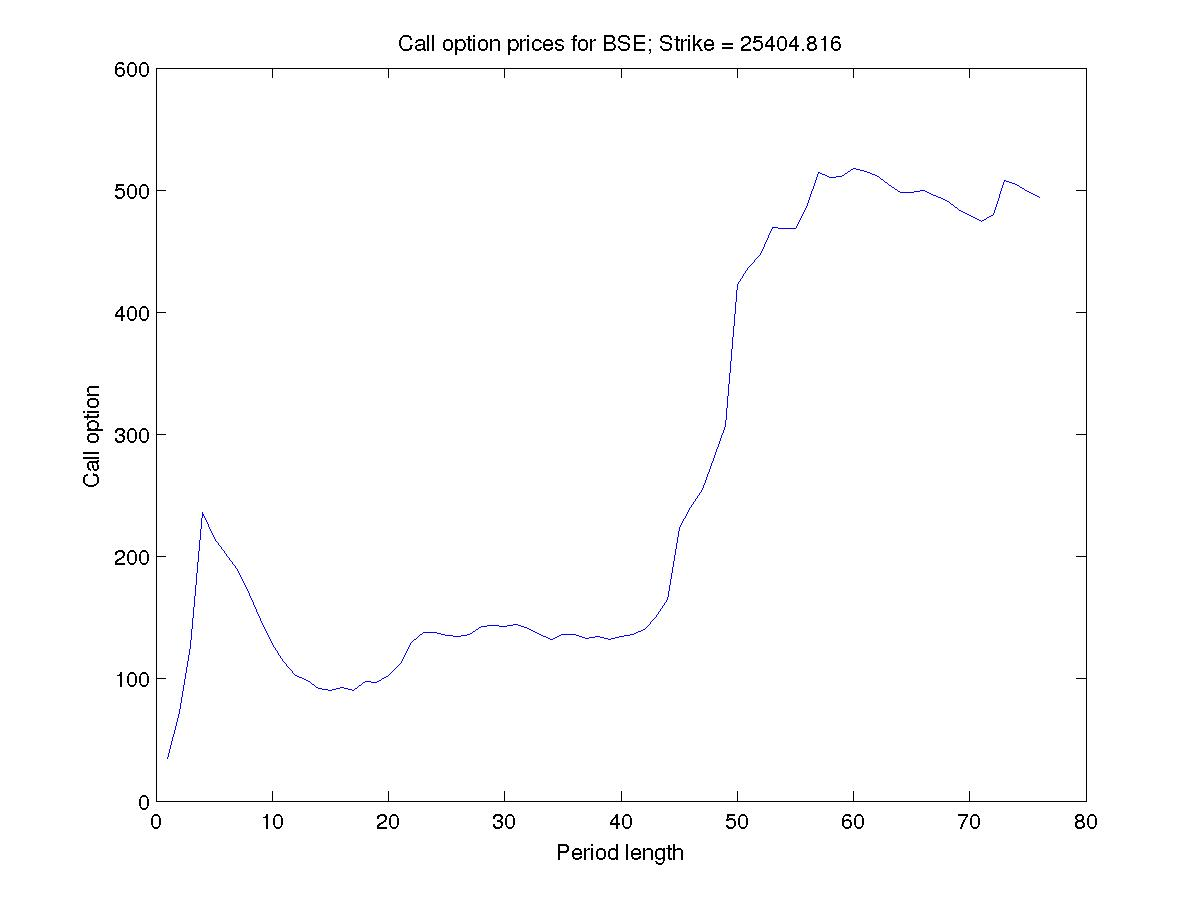
\includegraphics[width=5in]{put_strike8.jpg}
      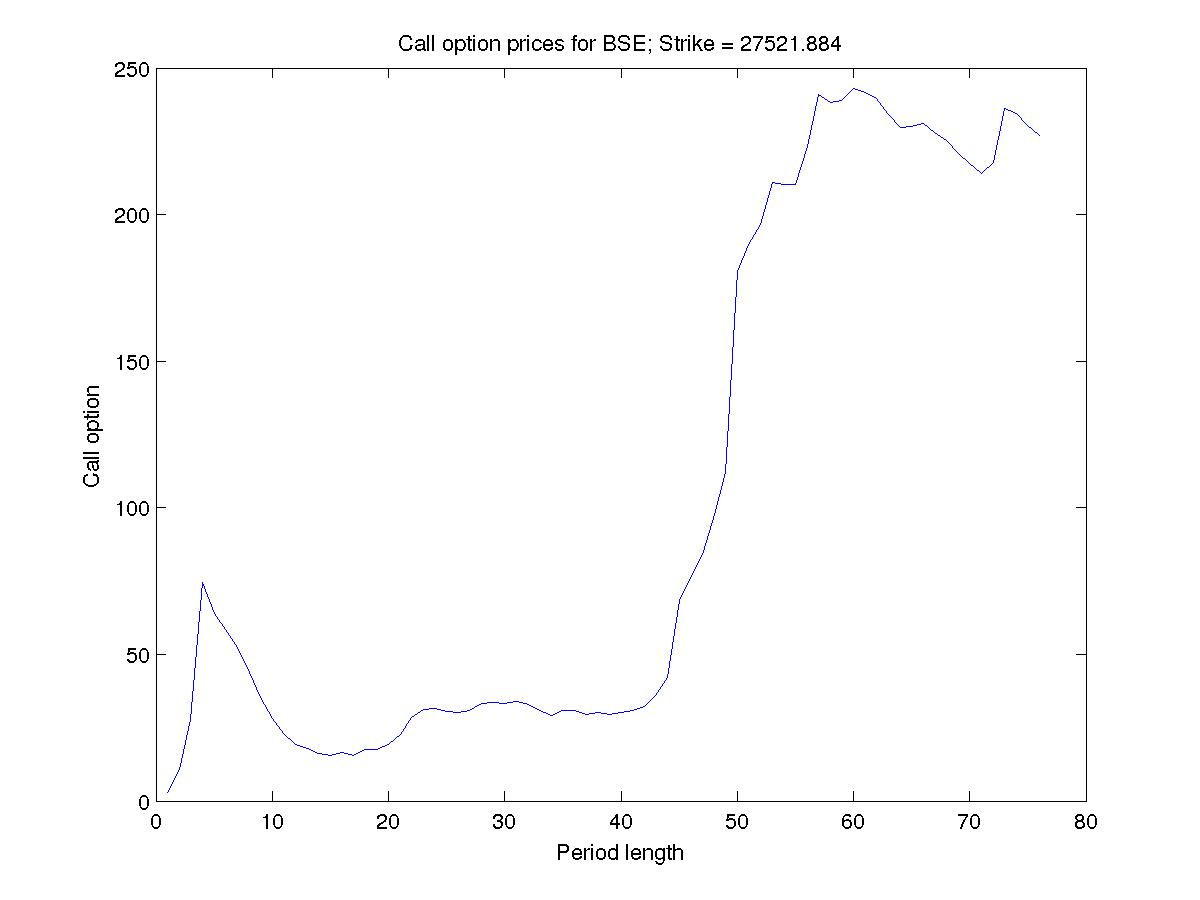
\includegraphics[width=5in]{put_strike9.jpg}
      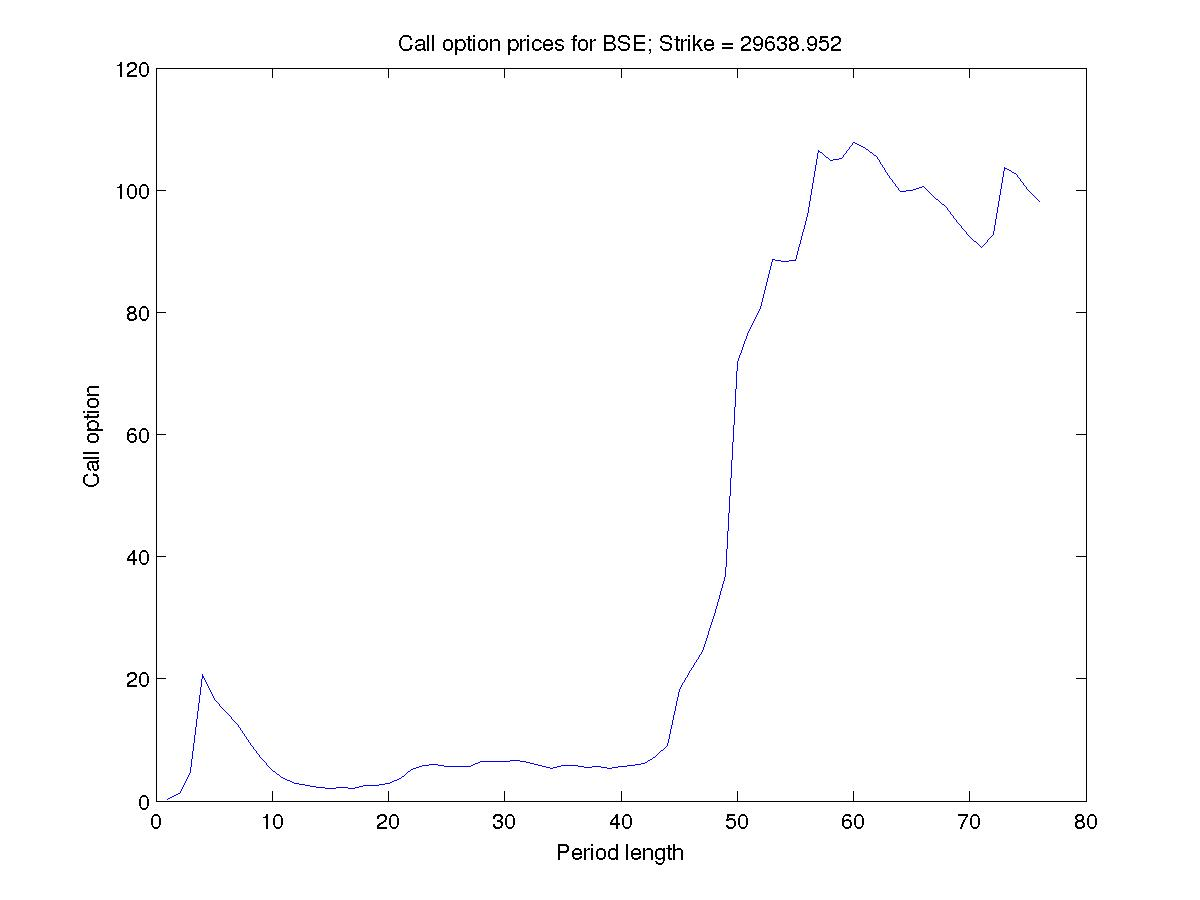
\includegraphics[width=5in]{put_strike10.jpg}
    \end{center}

\section{Code}
  \section{Function to compute Option price in BSM}
    \lstinputlisting{bsmoptionprice.m}
  \section{Driver program}
    \lstinputlisting{lab8.m}
\end{document}
